\label{sec:theory}
% Theoretical arguments in the literature closely related to your study
In this section we briefly introduce the market for commercial air transport in relation to network theory. We discuss how prices are determined and why network characteristics could potentially affect prices. This is followed by a short description of the network theory most pertinent to our analysis, and the measures we use to characterize the network and expand the feature set for the predictive model. The last subsection describes how we build a prediction model. 


%We draw on network theory to characterize how airports are connected to each other and analyze what role the individual airport plays in the network of airports. The ultimate aim of this analysis is to assess whether flight prices between airports depend on the role each airport plays in the network.\par
%We view airports as nodes in the network, with flights (or connections) representing links between airport. In connecting the network theory to the reality of the air transport market we use the terms interchangeably. Two airports are linked if there is at least one commercial flight between them in the time frame considered.

\subsection{Airline business models}
As outlined in the background in section \ref{subsec:b_deregulation} the common view is that large airlines specialize in either of two mayor business models with very different network characteristics. The traditional view within academia is that legacy airlines lean towards the hub-and-spoke network while low cost carriers (LCC) lean towards point-to-point connections \citep{daraban2012low,baker2013service,marti2015efficiency}.
\par
A third business model can be added, used by smaller regional airlines mainly serving the so-called spokes \citep{forbes2007role}, usually serving as a part of a hub-and-spoke network, though possibly also connecting spokes or offering a few longer-range connections to focus cities. Thus, we refine our common definitions by distinguishing between whether point-to-point connections are between spokes or focus cities.

\subsubsection{Point-to-point connections}
Point-to-point connections are direct connections between two nodes. In aviation terminology it is routes connecting airports by non-stop flights as opposed to transfers. One extreme is the fully-connected network in which every node is directly connected to each of the other nodes meaning that the number of links grows exponentially with the number of nodes such that the number of links are
\begin{equation*}
  l=\frac{n(n-1)}{2}
\end{equation*}
That is, a fully-connected network of 9 nodes would have no less than 36 links as seen in the left panel of Figure \ref{fig:different_networks}.

\subsubsection{Hub-and-spoke network}
The other extreme would be the single-hub network where $n$ nodes would only need $n-1$ connections as the $n-1$ non-hub nodes, so called spokes, would
 \par
\citet{o1987quadratic} presented a hub-and-spoke network as a simple single-assignment model such that non-hub nodes only have one edge, namely the one connecting them to a hub.


\begin{figure}[H]
  \centering
  \caption{Fully-connected point-to-point network vs hub-and-spoke network}
    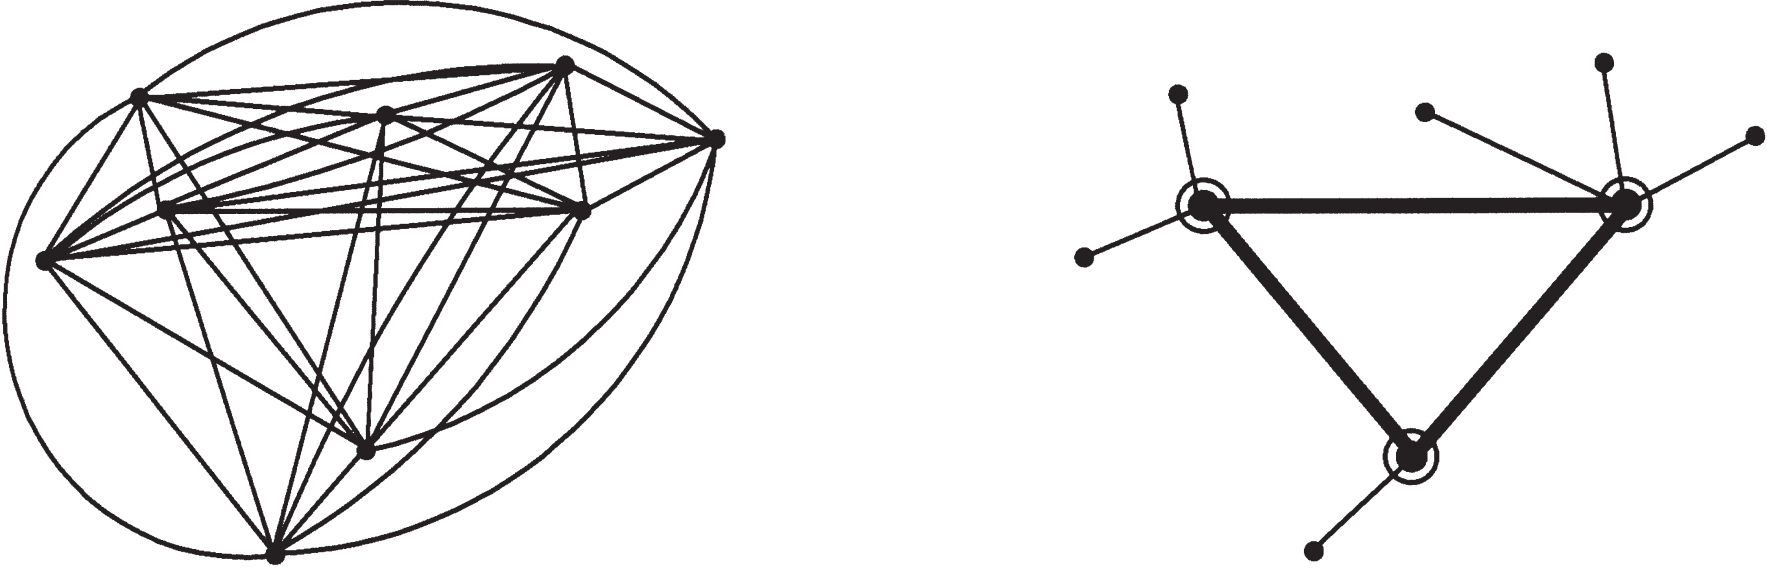
\includegraphics[width=1. \textwidth]{03_figures/Bryan_1999_networks}
    \sourcecenter{\citet{bryan1999hub}}
  \label{fig:different_networks}
\end{figure}

\subsubsection{Spokes vs focus nodes}
\citet{o1987quadratic} presented a hub-and-spoke network as a simple single-assignment model such that non-hub nodes only have one edge, namely the one connecting them to a hub. Thus, a single-hub route network connecting $n$ nodes would only need $n-1$ routes
A hub-and-spoke network

\subsection{Network Theory}
\label{subsec:Network Theory}
We draw on network theory to characterize how airports are connected to each other and analyze what role the individual airport plays in the network of airports. %The ultimate aim of this analysis is to assess whether flight prices between airports depend on the role each airport plays in the network. \\

\subsubsection{Network Characteristics}
\subsubsection{Air transport as a scale-free network}
A scale-free network is a network whose degree distribution follows a power law, i.e.: $p_k \sim k^{-\gamma}$. One characteristic of the scale-free networks is the existence of 'hubs' - nodes that have a far higher degree than the average degree. Air transport is - quite literally - a textbook example of a scale-free network, see chapter 4 of \citet{Barabasi}. As we will see in section \ref{sec:empirical}, this is reflected in the degree distribution, where most nodes have a low degree, but some nodes (hubs) have a very high degree.

Given this \textit{spoke-and-hub} nature of air transport, we expect the network to have some number of airports that are connected to all or most airports in its geographical vicinity, and well connected to similar airports in other regions. This pattern may be repeating to some extent, insofar as there may be regional, national and international hubs, depending on the size of the country. \\ 
\medskip
We further expect the network to be sparse, i.e. that the number of links is (far) lower than the number of possible links. This also reflects the hub-and-spoke nature of the network, in that small local airports are likely to have a low number of links, particularly relative to the possible number of links. We further expect the network to be connected, in the sense that, given an appropriate time frame, there will always be a path from one airport to the other (through some number of other airports).

\subsubsection{A Directed or Undirected Network}
Although individual flights are clearly directed, going from one airport to the other, we will primarily view the network as undirected. The reason being, that connections between airports are typically undirected.

As we will see in the data analysis, flights from airport i to airport j, almost always implies flights from airport j to airport i. We believe that this approach to the network of airports is well suited for our analysis, that focuses exclusively on the effect on prices. An analysis of e.g. how delays propagate through the network, would require viewing links as directed and including time in a more intricate manner.\\

\subsubsection{Weighted Network and Temporal Considerations}
In our analysis, we view the network as unweighted, i.e. all edges are considered equal. While this somewhat simplifies the analysis, we could have chosen to weight edges e.g. by letting the number of flights between two airports determine the 'weight' of their common edge. 
\medskip \\
The considered time frame clearly matters for the characteristics of the network, since not all flights between airports take place every day or even every week. Considering a years worth of flights will produce far more links in the network than considering the flights that take place on a particular day. We choose to analyze the yearly network, to ensure that we also capture flights (edges) that are seasonal in nature, e.g. flights that only happen in the summertime, or close to specific holidays. 

\subsubsection{Selected Network Measures}
In the course of the analysis, we draw upon a variety of measures to characterize the network. In the choice of measures, we look to \citet{chi2004structural}. The measures we have chosen to use are presented below. They are: Average degree, clustering coefficient, diameter, average shortest path length and betweenness centrality.


\paragraph{Average Degree}\mbox{} \\

The degree of node \textit{i} is the number of nodes with which node \textit{i} share an edge. In our cases, the degree of an airport is the number of airports to which it has flights (or that have flights to itself). 
The average degree is then simply the average across nodes. Average degree is calculated as: 
\begin{align}
    \text{Average degree} = \frac{1}{N} \sum_{i = 1}^N k_i = \frac{2L}{N}
\end{align}
\medskip
\paragraph{Clustering Coefficient} \mbox{} \\
The clustering coefficient for a given node \textit{i} is given as: 
\begin{align}
    C_i = \frac{2L_i}{k_i(k_i-1)}
    \intertext{Where $L_i$ denotes the number of links between node \textit{i}'s neighbors. The clustering coefficient of the network is then given by:}
    C = \frac{1}{N} \sum^N_{i=1} C_i
\end{align}
The clustering coefficient for a single node is equal to the fraction of possible edges between node \textit{i}'s neighbors (nodes it is connected to) that are found in the network. A node whose neighbors are all connected to each other will have a clustering coefficient of 1. Conversely, if none of the nodes neighbors are connected, it will have a clustering coefficient of 0. Note, that for nodes with degree 1, the clustering coefficient is 0. 
\medskip
\paragraph{Average Shortest Path Length}\mbox{} \\
The average shortest path length is defined as: 
\begin{align}
    a = \sum_{s,t \in V} \frac{d(s,t)}{N(N-1)}
\end{align}
Where V is the set of nodes in the network, and N is the number of nodes.
\paragraph{Diamater} \mbox{} \\
The diameter is the maximum shortest path length between any two nodes in the network. 
\medskip
\paragraph{Betweenness Centrality}\mbox{} \\
Finally, we also calculate the betweenness centrality. For node \textit{i}, this is the fraction of shortest paths between all nodes in the network that pass through node \textit{i}, \citep{brandes2008variants}.

\subsection{Prediction Model}
\label{subsec: prediction model}
Based on the available data we want to assess whether network characteristics can improve a prediction model predicting flight prices. The simplest way of predicting a continuous variable is to use a linear regression model. We write our prediction model as
$$
y_i = w_0 + W X_i 
$$
where $y_i$ is the price of a given flight, $w_0$ is the bias/intercept, $X_i$ is a vector of features, and $W$ is a vector of corresponding weights. 

To find the weights that makes the most accurate predictions we need to define a cost function. The standard cost function estimating a linear model is the \textbf{Mean Squared Error (MSE)}:
\begin{align}
\text{MSE}=\frac{1}{N} \sum_i^N (y_i - (w_0 + WX_i))^2
\end{align}
To address the problem of overfitting, we regularize the model using elastic net, which combines L1 ("Lasso") and L2 ("Ridge") regularization. Each of these regularization methods work by adding a term to the cost function. In the case of Lasso, the cost function then becomes: 
\begin{align}
    J(w) = \sum^N_{i=1} (y_i-\hat{y}_i)^2 + \alpha \cdot \sum_{j=1}^p |w_j|
    \intertext{where $p$ is the number of features in the model. The hyper-parameter $\alpha$ then controls the strength of the regularization. In the case of Ridge regularization, the cost function becomes:}
     J(w) = \sum^N_{i=1} (y_i-\hat{y}_i)^2 + \alpha \cdot \sum_{j=1}^p w_j^2
\end{align}
Ridge regularization shrinks the weights in the model. Lasso on the other hand tends to drive some coefficients to zero. \\
Elastic net combines the two regularization methods, and adds an additional hyperparameter, the L1-ratio, that determines the relative importance of Ridge- and Lasso regularization. The model is numerically optimized using gradient descent. \\ 

\subsubsection{Model evaluation}
In order to evaluate how our model performs on new data we start by splitting the data into a training set and test set. 
The model is estimated using k-fold cross validated grid search. When estimating the model we are only using the training data. This allows us to get an unbiased estimate of the performance when we evaluate the model on  the test data.
Estimating the model consists of two parts: one is to find the optimal weights in our prediction model - the other is to choose the optimal hyperparameters. The k-fold cross-validation randomly splits the training data into k folds, and then uses k-1 folds to train the model, that is optimizing the model, and evaluates performance on the last fold. This procedure is then repeated k times, so that we obtain k models and the resulting score is an average of these k models. This k-fold cross-validation is done for each set of hyperparameter in the Cartasian product of the hyperparameters and the set of hyperparameters that performs the best are chosen. Finally, the model is evaluated on the test data.
%Notes:



